\section{Results}
\label{sec:results}

Table~\ref{tab:rouge} and Figure~\ref{fig:rouge} report ROUGE against the
customer-written headline on the 300 held-out reviews. We state the outcomes
here and defer their interpretation to Section~\ref{sec:analysis}.

\begin{table}[t]
\caption{ROUGE on 300 held-out reviews. Best in bold.}
\label{tab:rouge}
\centering
\begin{tabular}{lccc}
\toprule
\textbf{Model} & \textbf{ROUGE-1} & \textbf{ROUGE-2} & \textbf{ROUGE-L} \\
\midrule
Lead-1 (extractive)        & 0.1255 & 0.0341 & 0.1145 \\
\texttt{t5-small}, not tuned & 0.1086 & 0.0266 & 0.0974 \\
\texttt{t5-small}, fine-tuned & \textbf{0.1751} & \textbf{0.0448} & \textbf{0.1723} \\
\bottomrule
\end{tabular}
\end{table}

\begin{figure}[t]
\centering
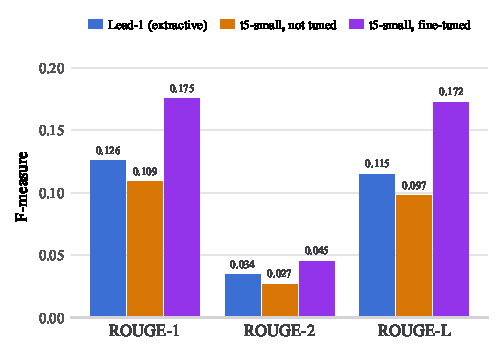
\includegraphics[width=\columnwidth]{figures/rouge_comparison.pdf}
\caption{ROUGE by model. The un-tuned pretrained model (centre) falls below the
extractive Lead-1 baseline (left) on all three measures.}
\label{fig:rouge}
\end{figure}

Three observations follow directly from the table.

\textbf{Fine-tuning helps substantially.} The fine-tuned model improves
ROUGE-1 from 0.1086 to 0.1751 over the same checkpoint untuned, a relative gain
of 61.2\%, with consistent gains on ROUGE-2 (+68.4\%) and ROUGE-L (+76.9\%).

\textbf{The task is not trivially extractive.} The fine-tuned model also beats
Lead-1, 0.1751 against 0.1255, a relative gain of 39.5\%. Lead-1 is a stronger
baseline than it may appear: customers frequently reuse their opening words in
their headline, so returning the first sentence captures real signal.

\textbf{The un-tuned pretrained model loses to Lead-1.} At 0.1086 against
0.1255 it scores 13.5\% below a baseline that performs no modelling at all, and
it does so on all three measures rather than on one. This is the result we
consider most informative, and Section~\ref{sec:analysis} takes it up.

Two properties of these numbers should be read carefully. First, all values are
low in absolute terms, and ROUGE-2 in particular sits near its floor; this is a
consequence of the reference length established in Section~\ref{sec:data} and
not, we argue, of the systems being uniformly poor. Second, \textbf{we ran no
significance test}, so we make no claim about whether any individual difference
would survive one. The 61.2\% and 13.5\% gaps are large relative to the values
involved, and the ordering is consistent across all three measures, but
consistency across correlated metrics is weak evidence and we do not present it
as more.

\subsection{Qualitative behaviour}

Table~\ref{tab:examples} pairs generated summaries with the customer headline
for four held-out reviews. The model produces short, headline-shaped output of
the register the task calls for. The final row is the informative failure: the
review praises a dog treat and then complains at length about the flatulence it
caused, and the model retains the praise while discarding the complaint.

\begin{table}[t]
\caption{Generated summaries against the customer's own headline.}
\label{tab:examples}
\centering
\begin{tabular}{p{0.44\columnwidth}p{0.42\columnwidth}}
\toprule
\textbf{Customer headline} & \textbf{Generated} \\
\midrule
totally worth the money!!! & he loves it! \\
i like this stuff!         & i love this cereal! \\
best i have found          & good taste, good quality \\
offensive gas producer!!!  & a great treat! \\
\bottomrule
\end{tabular}
\end{table}
